\documentclass[twoside,11pt,openright]{report}

\usepackage[latin1]{inputenc}
\usepackage[american]{babel}
\usepackage{a4}
\usepackage{latexsym}
\usepackage{amssymb}
\usepackage{amsmath}
\usepackage{epsfig}
\usepackage[T1]{fontenc}
\usepackage{mathptmx}
\usepackage{color}
\usepackage{epstopdf}
\usepackage{microtype}
\usepackage{hyperref}
\usepackage[useregional]{datetime2}
\DTMlangsetup[en-US]{showdayofmonth=false}
\usepackage{lipsum}
\usepackage{caption}
\usepackage{subcaption}
\usepackage{iris}
\usepackage{heaplang}
\usepackage{tikz}
\usetikzlibrary{calc,shapes.multipart,chains,arrows}

\renewcommand*\sfdefault{lmss}
\renewcommand*\ttdefault{txtt}

% Theorems, Corollaries, and Lemmas
\newtheorem{theorem}{Theorem}
\newtheorem{corollary}{Corollary}[theorem]
\newtheorem{lemma}[theorem]{Lemma}

\newtheorem{definition}{Definition}[section]


\newcommand{\isLock}{\operatorname{isLock}}
\newcommand{\locked}{\operatorname{locked}}
\newcommand{\issued}{\operatorname{issued}}
\newcommand{\newLock}{\operatorname{newLock}}
\newcommand{\acquire}{\operatorname{acquire}}
\newcommand{\wait}{\operatorname{wait}}
\newcommand{\release}{\operatorname{release}}
\newcommand{\lockInv}{\operatorname{lockInv}}
\newcommand{\initialise}{\operatorname{initialize}}
\newcommand{\enqueue}{\operatorname{enqueue}}
\newcommand{\dequeue}{\operatorname{dequeue}}

\newcommand{\isqueue}{\operatorname{is\_queue}}

\newcommand{\isLLchain}[1]{\operatorname{isLL\_chain} \; #1}
\newcommand{\isLL}{\operatorname{isLL}}

\newcommand{\locin}[1]{\loc_{#1\_\text{in}}}
\newcommand{\locout}[1]{\loc_{#1\_\text{out}}}

\newcommand{\nIn}[1]{\operatorname{in} \; #1}
\newcommand{\nVal}[1]{\operatorname{val} \; #1}
\newcommand{\nOut}[1]{\operatorname{out} \; #1}

\newcommand\catenate{\mathbin{\text{\ttfamily\upshape ++}}}

\newcommand{\todo}[1]{{\color[rgb]{.5,0,0}\textbf{$\blacktriangleright$#1$\blacktriangleleft$}}}

\begin{document}

%%%%%%%%%%%%%%%%%%%%%%%%%%%%%%%%%%%%%%%%%%%%%%%%%%%%%%%%%%%%%%%%%%%%%%%

\pagestyle{empty}
\pagenumbering{roman} 
\vspace*{\fill}\noindent{\rule{\linewidth}{1mm}\\[4ex]
{\Huge\sf TITLE HERE}\\[2ex]
{\huge\sf Mathias Pedersen, 201808137}\\[2ex]
\noindent\rule{\linewidth}{1mm}\\[4ex]
\noindent{\Large\sf Master's Thesis, Computer Science\\[1ex] 
\today \\[1ex] Advisor: Amin Timany\\[15ex]}\\[\fill]}

\epsfig{file=logo.eps}\clearpage

%%%%%%%%%%%%%%%%%%%%%%%%%%%%%%%%%%%%%%%%%%%%%%%%%%%%%%%%%%%%%%%%%%%%%%%

\pagestyle{plain}
\chapter*{Abstract}
\addcontentsline{toc}{chapter}{Abstract}

\todo{in English\dots}

\chapter*{Resum\'e}
\addcontentsline{toc}{chapter}{Resum\'e}

\todo{in Danish\dots}

\chapter*{Acknowledgments}
\addcontentsline{toc}{chapter}{Acknowledgments}

\todo{\dots}

\vspace{2ex}
\begin{flushright}
  \emph{Mathias Pedersen}\\
  \emph{Aarhus, \today.}
\end{flushright}

\tableofcontents
\cleardoublepage
\pagenumbering{arabic}
\setcounter{secnumdepth}{2}

%%%%%%%%%%%%%%%%%%%%%%%%%%%%%%%%%%%%%%%%%%%%%%%%%%%%%%%%%%%%%%%%%%%%%%%

\chapter{Introduction}
\label{ch:intro}

\todo{motivate and explain the problem to be addressed}

\todo{example of a citation: \cite{DBLP:conf/podc/MichaelS96}}
\todo{get your bibtex entries from \url{https://dblp.org/}}

%%%%%%%%%%%%%%%%%%%%%%%%%%%%%%%%%%%%%%%%%%%%%%%%%%%%%%%%%%%%%%%%%%%%%%%

\chapter{The Great Ideas}
\label{ch:main}

The Two-Lock Michael Scott Queue

I present here he an implementation of the Two-lock MS-Queue in HeapLang. This implementation differs slightly from the original, presented in \cite{DBLP:conf/podc/MichaelS96}, but most changes simply reflect the differences in the two languages.


Preliminaries

The underlying data structure making up the queue is a singly-linked list. The linked-list will always contain at least one element, called the \emph{sentinel} node, marking the beginning of the queue. Note that the sentinel node is itself not part of the queue, but all nodes following it are. The queue keeps a head pointer ($\loc_{head}$) which always points to the sentinel, and a tail pointer ($\loc_{tail}$) which points to some node in the linked list.

In my implementation, a node can be thought of as a triple $(\locin{i}, v_i, \locout{i})$. The location $\locin{i}$ points to the pair $(v_i, \locout{i})$, where $v_i$ is the value of the node, and $\locout{i}$ either points to $\None$ which represents the null pointer, or to the next node in the linked list. When we say that a location $\loc$ points to a node $(\locin{i}, v_i, \locout{i})$, we mean that $\loc \mapsto \locin{i}$. Hence, if we have two adjacent nodes $(\locin{i}, v_i, \locout{i})$, $(\locin{i+1}, v_{i+1}, \locout{i+1})$ in the linked list, then we have the following structure: $\locin{i} \mapsto (v_i, \locout{i})$, $\locout{i} \mapsto \locin{i+1}$, and $\locin{i+1} \mapsto v_{i+1}, \locout{i+1}$.

The reader may wonder why there is an extra, intermediary "in" pointer, between the pairs of the linked list, and why the "out" pointer couldn't point directly to the next pair. In the original implementation \cite{DBLP:conf/podc/MichaelS96}, nodes are allocated on the heap. To simulate this in HeapLang, when creating a new node, we create a pointer to a pair making up the node. Now, in the C-like language used in the original specification, an assignment operator is available which is not present in HeapLang. So in order to mimic this behaviour, we model variables as pointers. In this way, we can model a variable $\lvarA$ as a location $\loc_{\lvarA}$, and the value stored at $\loc_{\lvarA}$ is the current value of $\lvarA$. This means that the variable $\locout{i}$ (called "next" in the original) becomes a location $\loc_{head}$, and the value stored at the location is what head is currently assigned to. Since $\locout{i}$ is supposed to be a variable containing a pointer, then the value saved at that location will also be a pointer.


The queue consists of 3 functions: $\initialise$, $\enqueue$, and $\dequeue$ which I now present in turn.

$\initialise$

$\initialise$ will first create a single node -- the sentinel -- marking the start of the linked list. It then creates two locks, $H\_lock$ and $T\_lock$, protecting the head and tail pointers, respectively. Finally, it creates the head and tail pointers, both pointing to the sentinel. The queue is then a pointer to a structure containing the head, the tail, and the two locks.\\
Figure \ref{MSQTL:impl:figure:init} illustrates the structure of the queue after initialisation. Note that one of the pointers is coloured blue. This represents a \emph{persistent} pointer; a pointer that will never be updated again. All "in" pointers $\locin{i}$, are persistent, meaning that they will always point to $(v_i, \locout{i})$. We shall use the notation $\loc \mapsto \square v$ (introduced in \cite{DBLP:conf/cpp/VindumB21}) to mean that $\loc$ points persistently to $v$.

Note that in the original specification, a queue is a pointer to a 4-tuple $(\loc_{head}, \loc_{tail}, H\_lock, T\_lock)$. Since HeapLang doesn't support 4-tuples, we instead represent the queue as a pointer to a pair of pairs: $((\loc_{head}, \loc_{tail}), (H\_lock, T\_lock))$.


$\enqueue$

To enqueue a value, we must create a new node, append it to the underlying linked-list, and swing the tail pointer to this new node. These three operations are depicted in figure \ref{MSQTL:impl:figure:enqueue}.

$\enqueue$ takes as argument the value to be enqueued and creates a new node containing this value (corresponding to figure \ref{MSQTL:impl:figure:enqueue:a}). This creation doesn't interact with the underlying queue data-structure, hence why we don't acquire the $T\_lock$ first. After creating the new node, we must make the last node in the linked list point to it. Since this operation interacts with the queue, we first acquire the $T\_lock$. Once we obtain the lock, we make the last node in the linked list point to our new node (figure \ref{MSQTL:impl:figure:enqueue:b}). Following this, we swing $\loc_{tail}$ to the new last node in the linked list (figure \ref{MSQTL:impl:figure:enqueue:c}).

Figure \ref{MSQTL:impl:figure:enqueue} also illustrates when pointers become persistent; once the previous last node is updated to point to the newly inserted node, that pointer will never be updated again, hence becoming persistent.


$\dequeue$

It is of course only possible to dequeue an element from the queue if the queue contains at least one element. Hence, the first thing $\dequeue$ does is check if the queue is empty. We can detect an empty queue by checking if the sentinel is the last node in the linked list. Being the last node in the linked list corresponds to having the "out" node be $\None$. If this is the case, then the queue is empty and the code returns $\None$. Otherwise, there is a node just after the sentinel, which is the first node of the queue. To dequeue it, we first read the associated value, and next we swing the head to it, making it the new sentinel. Finally, we return the value we read.

Since all of these operations interact with the queue, we shall only perform them after having acquired $H\_lock$.

Figure \ref{MSQTL:impl:figure:dequeue} illustrates running dequeue on a non-empty queue. Note that the only change is that the head pointer is swung to the next node in the linked list; the old sentinel is not deleted, it just become unreachable from the heap pointer. In this way, the linked list only ever grows.

\begin{figure}[h]
  \centering
  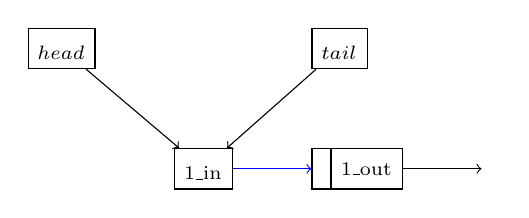
\begin{tikzpicture}[
    pair/.style = {
      on chain,
      rectangle split,
      rectangle split horizontal,
      rectangle split parts=2,
      draw,
      anchor=center,
      text height=1.5ex,
    },
    perspointer/.style = {
      on chain,
      rectangle,
      draw,
      anchor=center,
      text height=1.5ex,
    },
    pointer/.style = {
      rectangle,
      draw,
      anchor=center,
      text height=1.5ex,
    },
    start chain=going right,
  ]

  % Linked List
  \node (l'1) [join={by ->}, perspointer,on chain] {$\locin{1}$};
  \node (l1pair) [join={by ->, draw=blue}, pair,on chain] {$\None$ \nodepart{two} $\locout{1}$};
  \node (null) [join={by ->, draw=black}, rectangle,on chain] {$\None$};

  % Head and tail
  \node (head) [pointer, above left=of l'1] {$\loc_{head}$};
  \node (tail) [pointer, above right=of l'1] {$\loc_{tail}$};
  \draw[->] (head) -- (l'1);
  \draw[->] (tail) -- (l'1);
  
  \end{tikzpicture}
  \caption{Queue after initialisation}
  \label{MSQTL:impl:figure:init}
\end{figure}


\begin{figure}[h]
  \centering
  \begin{subfigure}{\textwidth}
    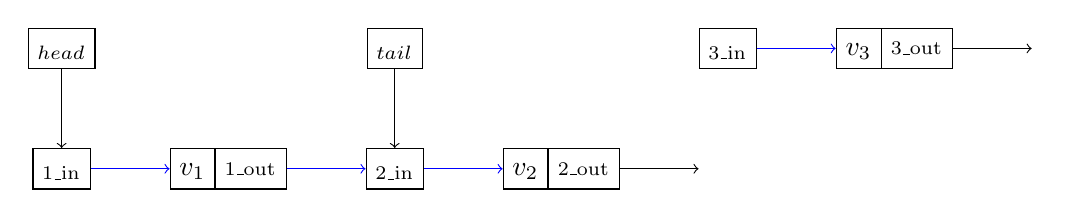
\begin{tikzpicture}[
      pair/.style = {
        on chain,
        rectangle split,
        rectangle split horizontal,
        rectangle split parts=2,
        draw,
        anchor=center,
        text height=1.5ex,
      },
      perspointer/.style = {
        on chain,
        rectangle,
        draw,
        anchor=center,
        text height=1.5ex,
      },
      pointer/.style = {
        rectangle,
        draw,
        anchor=center,
        text height=1.5ex,
      },
      start chain=going right,
    ]
  
    % Linked List
    \node (l'1) [join={by ->}, perspointer,on chain] {$\locin{1}$};
    \node (l1pair) [join={by ->, draw=blue}, pair,on chain] {$v_1$ \nodepart{two} $\locout{1}$};
    \node (l'2) [join={by ->, draw=blue}, perspointer,on chain] {$\locin{2}$};
    \node (l2pair) [join={by ->, draw=blue}, pair,on chain] {$v_2$ \nodepart{two} $\locout{2}$};
    \node (null) [join={by ->, draw=black}, rectangle,on chain] {$\None$};
  
    \node (l'3) [perspointer, above right=of l2pair] {$\locin{3}$};
    \node (l3pair) [join={by ->, draw=blue}, pair,on chain] {$v_3$ \nodepart{two} $\locout{3}$};
    \node (null) [join={by ->, draw=black}, rectangle,on chain] {$\None$};
  
    % Head and tail
    \node (head) [pointer, above=of l'1] {$\loc_{head}$};
    \node (tail) [pointer, above=of l'2] {$\loc_{tail}$};
    \draw[->] (head) -- (l'1);
    \draw[->] (tail) -- (l'2);
    
    \end{tikzpicture}
    \caption{Queue after creating the new node $(\locin{3}, v_3, \locout{3})$ to be added to the queue.}
    \label{MSQTL:impl:figure:enqueue:a}
    \vspace{2em}
  \end{subfigure}
  \begin{subfigure}{\textwidth}
    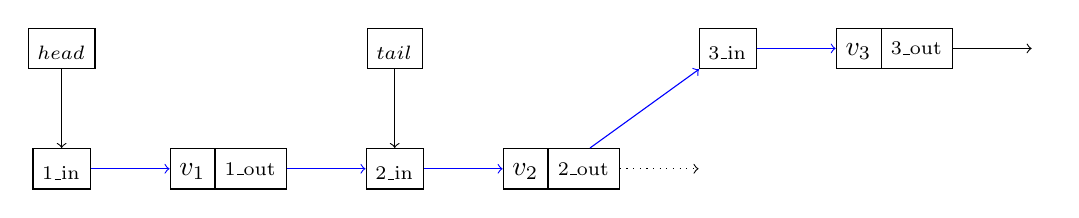
\begin{tikzpicture}[
      pair/.style = {
        on chain,
        rectangle split,
        rectangle split horizontal,
        rectangle split parts=2,
        draw,
        anchor=center,
        text height=1.5ex,
      },
      perspointer/.style = {
        on chain,
        rectangle,
        draw,
        anchor=center,
        text height=1.5ex,
      },
      pointer/.style = {
        rectangle,
        draw,
        anchor=center,
        text height=1.5ex,
      },
      start chain=going right,
    ]
  
    % Linked List
    \node (l'1) [join={by ->}, perspointer,on chain] {$\locin{1}$};
    \node (l1pair) [join={by ->, draw=blue}, pair,on chain] {$v_1$ \nodepart{two} $\locout{1}$};
    \node (l'2) [join={by ->, draw=blue}, perspointer,on chain] {$\locin{2}$};
    \node (l2pair) [join={by ->, draw=blue}, pair,on chain] {$v_2$ \nodepart{two} $\locout{2}$};
    \node (null) [join={by ->, dotted, draw=black}, rectangle,on chain] {\textcolor{gray}{$\None$}};
  
    \node (l'3) [perspointer, above right=of l2pair] {$\locin{3}$};
    \node (l3pair) [join={by ->, draw=blue}, pair,on chain] {$v_3$ \nodepart{two} $\locout{3}$};
    \node (null) [join={by ->, draw=black}, rectangle,on chain] {$\None$};
    \draw[->, draw=blue] (l2pair) -- (l'3);
  
    % Head and tail
    \node (head) [pointer, above=of l'1] {$\loc_{head}$};
    \node (tail) [pointer, above=of l'2] {$\loc_{tail}$};
    \draw[->] (head) -- (l'1);
    \draw[->] (tail) -- (l'2);
    
    \end{tikzpicture}
    \caption{Queue after adding the new node to linked list.}
    \label{MSQTL:impl:figure:enqueue:b}
    \vspace{2em}
  \end{subfigure}
  \begin{subfigure}{\textwidth}
    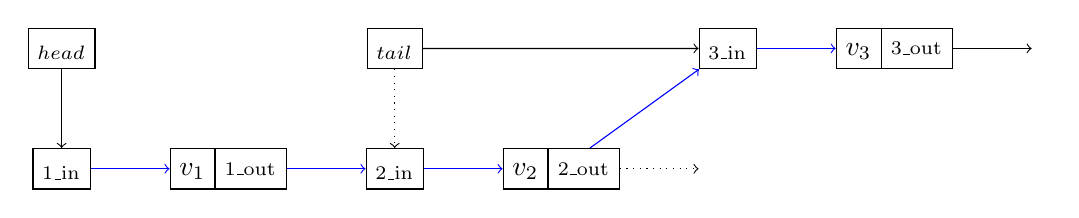
\begin{tikzpicture}[
      pair/.style = {
        on chain,
        rectangle split,
        rectangle split horizontal,
        rectangle split parts=2,
        draw,
        anchor=center,
        text height=1.5ex,
      },
      perspointer/.style = {
        on chain,
        rectangle,
        draw,
        anchor=center,
        text height=1.5ex,
      },
      pointer/.style = {
        rectangle,
        draw,
        anchor=center,
        text height=1.5ex,
      },
      start chain=going right,
    ]
  
    % Linked List
    \node (l'1) [join={by ->}, perspointer,on chain] {$\locin{1}$};
    \node (l1pair) [join={by ->, draw=blue}, pair,on chain] {$v_1$ \nodepart{two} $\locout{1}$};
    \node (l'2) [join={by ->, draw=blue}, perspointer,on chain] {$\locin{2}$};
    \node (l2pair) [join={by ->, draw=blue}, pair,on chain] {$v_2$ \nodepart{two} $\locout{2}$};
    \node (null) [join={by ->, dotted, draw=black}, rectangle,on chain] {\textcolor{gray}{$\None$}};
  
    \node (l'3) [perspointer, above right=of l2pair] {$\locin{3}$};
    \node (l3pair) [join={by ->, draw=blue}, pair,on chain] {$v_3$ \nodepart{two} $\locout{3}$};
    \node (null) [join={by ->, draw=black}, rectangle,on chain] {$\None$};
    \draw[->, draw=blue] (l2pair) -- (l'3);
  
    % Head and tail
    \node (head) [pointer, above=of l'1] {$\loc_{head}$};
    \node (tail) [pointer, above=of l'2] {$\loc_{tail}$};
    \draw[->] (head) -- (l'1);
    \draw[->, dotted] (tail) -- (l'2);
    \draw[->] (tail) -- (l'3);
    
    \end{tikzpicture}
    \caption{Queue after swinging tail pointer to the new node.}
    \label{MSQTL:impl:figure:enqueue:c}
  \end{subfigure}
  \caption{Enqueuing an element to a queue with one element.}
  \label{MSQTL:impl:figure:enqueue}
\end{figure}


\begin{figure}[h]
  \centering
  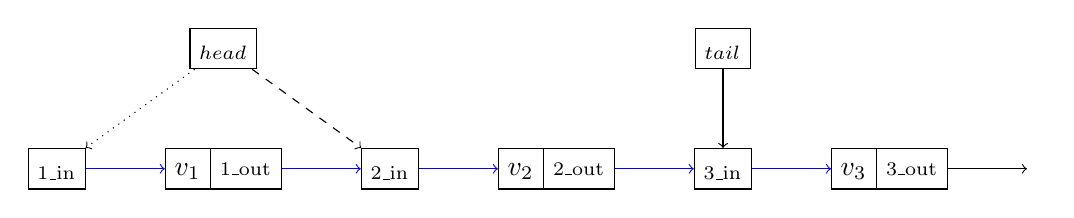
\begin{tikzpicture}[
    pair/.style = {
      on chain,
      rectangle split,
      rectangle split horizontal,
      rectangle split parts=2,
      draw,
      anchor=center,
      text height=1.5ex,
    },
    perspointer/.style = {
      on chain,
      rectangle,
      draw,
      anchor=center,
      text height=1.5ex,
    },
    pointer/.style = {
      rectangle,
      draw,
      anchor=center,
      text height=1.5ex,
    },
    start chain=going right,
  ]

  % Linked List
  \node (l1in) [join={by ->}, perspointer,on chain] {$\locin{1}$};
  \node (l1pair) [join={by ->, draw=blue}, pair,on chain] {$v_1$ \nodepart{two} $\locout{1}$};
  \node (l2in) [join={by ->, draw=blue}, perspointer,on chain] {$\locin{2}$};
  \node (l2pair) [join={by ->, draw=blue}, pair,on chain] {$v_2$ \nodepart{two} $\locout{2}$};
  \node (l3in) [join={by ->, draw=blue}, perspointer,on chain] {$\locin{3}$};
  \node (l3pair) [join={by ->, draw=blue}, pair,on chain] {$v_3$ \nodepart{two} $\locout{3}$};
  \node (null) [join={by ->, draw=black}, rectangle,on chain] {$\None$};

  % Head and tail
  \node (head) [pointer, above=of l1pair] {$\loc_{head}$};
  \node (tail) [pointer, above=of l3in] {$\loc_{tail}$};
  \draw[->, dotted] (head) -- (l1in);
  \draw[->, dashed] (head) -- (l2in);
  \draw[->] (tail) -- (l3in);
  
  \end{tikzpicture}
  \caption{Dequeueing an element ($v_2$) from a queue with two elements ($v_2$, $v_3$). The dotted line represents the state before the dequeue, and the dashed line is the state after dequeuing.}
  \label{MSQTL:impl:figure:dequeue}
\end{figure}


\begin{align*}
  \langkw{let} \initialise := &\\
                    & \Let node = \Ref((\None, \Ref(\None))) in\\
                    & \Let H\_lock = newlock \TT in\\
                    & \Let T\_lock = newlock \TT in\\
                    & \Ref ((\Ref(node), \Ref(node)), (H\_lock, T\_lock))
\end{align*}

\begin{align*}
  \langkw{let} \enqueue \ Q \ value :=&\\
		& \Let node = \Ref ((\Some value, \Ref(\None))) in\\
		& \acquire (\Snd (\Snd (\deref Q)));\\
		& \Snd (\deref(\deref(\Snd (\Fst(\deref Q))))) \gets node;\\
		& \Snd (\Fst (\deref Q)) \gets node;\\
		& \release (\Snd (\Snd (\deref Q)))
\end{align*}

\begin{align*}
  \langkw{let} \dequeue \ Q :=&\\ 
		& \acquire (\Fst (\Snd (\deref Q)));\\
		& \Let node = \deref (\Fst (\Fst (\deref Q))) in\\
		& \Let new\_head = \deref (\Snd(\deref node)) in\\
		& \If new\_head = \None then\\
			& \hspace{20pt} \release (\Fst (\Snd(\deref Q)));\\
			& \hspace{20pt} \None\\
		& \Else\\
			& \hspace{20pt} \Let value = \Fst (\deref new\_head) in\\
			& \hspace{20pt} \Fst (\Fst (\deref Q)) \gets new\_head;\\
			& \hspace{20pt} \release (\Fst (\Snd (\deref Q)));\\
      & \hspace{20pt} value
\end{align*}


Sequential Specification

\begin{align*}
  &\exists \isqueue : \Val \to \List (\Loc \times \Val \times \Loc) \to Qgnames \to \Prop.\\
  &\quad\quad\hoare{\TRUE}{\initialise \TT}{v . \exists Q_\gname, \isqueue\ v\ []\ Q_\gname}\\
  &\land\quad\forall q, v, xs, Q_\gname. \hoare{\isqueue \; v \; xs \; Q_\gname}{\enqueue\ q\ v}{v . \exists x, \nVal{x} = \Some v \ast \isqueue\ q\ (x :: xs)\ Q_\gname}\\
  &\land\quad\forall q, v, xs, Q_\gname. \hoare{\isqueue \; v \; xs \; Q_\gname}{\dequeue\ q}{v . \begin{array}{l}(xs = [] \ast v = \None \ast \isqueue\ q\ xs\ Q_\gname) \; \lor\\ (\exists x, xs'. xs = xs' \catenate [x] \ast v = \nVal{x} \ast \isqueue\ q\ xs'\ Q_\gname) \end{array}}
\end{align*}


\begin{definition}[Linked List Chain Predicate]
  \begin{align*}
    \isLLchain{[]} \equiv& \TRUE\\
    \isLLchain{[x]} \equiv& \nIn{x} \mapsto\square (\nVal{x}, \nOut{x})\\
    \isLLchain{x :: x' :: xs} \equiv& \nIn{x} \mapsto\square (\nVal{x}, \nOut{x}) \ast \nOut{x'} \mapsto\square \nIn{x} \ast \isLLchain{x' :: xs}
  \end{align*}
\end{definition}

\begin{definition}[Linked List Predicate]
  \begin{align*}
    \isLL{[]} \equiv& \TRUE\\
    \isLL{x :: xs} \equiv& \nOut{x} \mapsto \None \ast \isLLchain{x :: xs}
  \end{align*}
\end{definition}

Key insights
\begin{enumerate}
  \item\label{MSQTL:insights:head} Head always points to the first node in the queue.
  \item\label{MSQTL:insights:tail} Tail always point to either the last or second last node in the queue.
  \item\label{MSQTL:insights:persistent} All but the last pointer in the queue (the pointer to null) never change
\end{enumerate}

Insight \ref{MSQTL:insights:tail} is true, as it holds initially, and every time a new node is enqueued, the tail pointer is updated to point to the last node, and no other nodes can be enqueue before the update takes place. However, just after the new node has been linked to the queue, the tail queue will be pointing to the second last node in the queue, until it is updated in the next line.

Insight \ref{MSQTL:insights:persistent} means that we can mark all pointers in the queue (except the pointer to the null node) as persistent.



Concurrent Specification

\begin{align*}
  &\exists \isqueue : \Val \mapsto Qgnames \mapsto \Prop.\\
  &\quad\quad\persistently (\forall v, Q_\gname . \isqueue \; v \; Q_\gname \implies \persistently \isqueue \; v \; Q_\gname)\\
  &\land\quad\hoare{\TRUE}{\initialise \TT}{v . \exists Q_\gname, \isqueue\ v\ Q_\gname}\\
  &\land\quad\forall q, v, Q_\gname. \hoare{\isqueue \; v \; Q_\gname}{\enqueue\ q\ v}{v . \TRUE}\\
  &\land\quad\forall q, v, Q_\gname. \hoare{\isqueue \; v \; Q_\gname}{\dequeue\ q}{v . \TRUE}
\end{align*}


Key insights (concurrent)
\begin{enumerate}
  \item All the same as before
  \item\label{MSQTL:insights:lag} The tail can lag one node behind Head
  \item\label{MSQTL:insights:states} At any given time, the queue is in one of four states:
    \begin{enumerate}
      \item\label{MSQTL:insights:state:static} No threads are interacting with the queue (\textbf{Static})
      \item\label{MSQTL:insights:state:enqueue} A thread is enqueueing (\textbf{Enqueue})
      \item\label{MSQTL:insights:state:dequeue} A thread is dequeuing (\textbf{Dequeue})
      \item\label{MSQTL:insights:state:both} A thread is enqueueing and a thread is dequeuing (\textbf{Both})
    \end{enumerate}
\end{enumerate}

Insight \ref{MSQTL:insights:lag} might seem a little surprising, and indeed it stands in contrast to property 5 in \cite{DBLP:conf/podc/MichaelS96}, which states that the tail never lags behind head. I also didn't realise this possibility until a proof attempt using a model that "forgot" old nodes lead to an unprovable case (see section \ref{MSQTL:Discussion:xs_old}). The situation can occur when the queue is empty, and a thread performs an incomplete enqueue; it attaches the new node to the end, but before it can swing the tail to this new node, another thread performs a dequeue, which dequeues this new node, swinging the head to it. Now the tail is lagging a node behind the head.

It is not possible for the tail to point more than one node behind the head, as in order for this to happen, more nodes must be enqueued, but this can't happen before the current enqueue finishes, which will update the tail and bring it up to speed with the head.

Fortunately, this isn't an issue for safety, but a consequence of this possibility is that when modelling the queue, we must remember at least one "old" node (i.e. a dequeued node), as the tail might be pointing to this node. For the sake of simplicity in the model, the choice is made to remember an arbitrary amount of old nodes, which is represented by the list $xs_{old}$.


With these insights, we can now define the queue invariant.

\begin{definition}[Two-Lock M\&S-Queue Invariant]\label{MSQTL:spec:invariant}
  \todo{Write it in}
\end{definition}

The specification for the two-lock Michael Scott Queue \textit{can} be proven using the queue invariant \ref{MSQTL:spec:invariant}. However, during the proof, a simpler (but arguably less intuitive) queue invariant was discovered This simpler invariant is equivalent to \ref{MSQTL:spec:invariant} and has the added benefit of being easier to work with in the proofs. Thus, we shall be using this version of the queue invariant during the proofs.

\begin{definition}[Simplified Two-Lock M\&S-Queue Invariant]\label{MSQTL:spec:invariant:simple}
  \todo{Write it in}
\end{definition}


\subsubsection{Discussing the need for $xs_{old}$}\label{MSQTL:Discussion:xs_old}

As mentioned in the insights, it is possible for the tail to lag one node behind the head. This insight lead to including the old nodes of the queue in the queue invariant. This addition manifests in the end of the proof of dequeue. When we open the invariant to swing the head to the new node, we get that the entire queue is $xs$. After performing the write, we can then close the invariant with the same $xs$ that we opened the queue to (just written differently to signify that $x_{head}$ is now "old"). Because of this, we can supply the same predicate concerning the $tail$ (the or) that we opened the queue with, since these only mention $xs$, which remains the same.

Had we not used an $xs_{old}$ and essentially just "forgotten" old nodes in the queue, we couldn't have done this. Say that we defined $xs$ as $xs = x_{head} :: xs_{rest}$ instead. Then, once we have to close the invariant, we cannot supply the $xs$, which we got when we opened the invariant. Our only choice (due to the fact that $head$ must point to $x_{n_head}$) is to close the invariant with $xs' = xs_{rest} = x_{n_head} :: xs_{n_rest}''$. However, clearly $xs' \neq xs$, so we cannot supply the same predicate concerning the $tail$ (the or) that we got when opening the invariant, since this predicate talks about $xs$, not $xs'$. Now, if we opened the invariant in the Dequeue case, then we could assert that $last xs = last xs'$, and hence still be able close the invariant. However, if we opened the invariant in the Both case, then we would need to assert that $2last xs = 2last xs'$. This is however not provable, since it might be the case that $xs_{n_rest}''$ is empty, and hence $2last xs'$ is $None$, whereas $2last xs = x_{n_head}$.


%%%%%%%%%%%%%%%%%%%%%%%%%%%%%%%%%%%%%%%%%%%%%%%%%%%%%%%%%%%%%%%%%%%%%%%

\chapter{Conclusion}
\label{ch:conclusion}

\todo{conclude on the problem statement from the introduction}

%%%%%%%%%%%%%%%%%%%%%%%%%%%%%%%%%%%%%%%%%%%%%%%%%%%%%%%%%%%%%%%%%%%%%%%

\cleardoublepage
\addcontentsline{toc}{chapter}{Bibliography}
\bibliographystyle{plain} 
\bibliography{refs}

%%%%%%%%%%%%%%%%%%%%%%%%%%%%%%%%%%%%%%%%%%%%%%%%%%%%%%%%%%%%%%%%%%%%%%%

\cleardoublepage
\appendix
\chapter{The Technical Details}

\todo{\dots}

\end{document}

